% =========================================================================
\chapter{How the warnings are scored}
\label{ch:metrics}
% =========================================================================

\section{The confusion matrix}
Every test row ends in one of four boxes:
\begin{center}
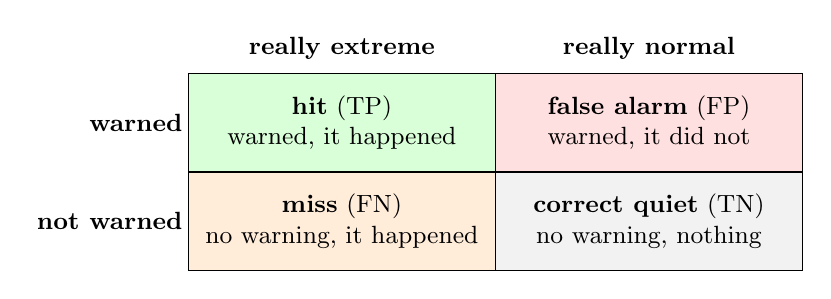
\begin{tikzpicture}[cell/.style={draw,minimum width=3.9cm,minimum height=1.25cm,align=center,font=\small}]
\node[cell,fill=green!15] at (0,0) {\textbf{hit} (TP)\\warned, it happened};
\node[cell,fill=red!12] at (3.9,0) {\textbf{false alarm} (FP)\\warned, it did not};
\node[cell,fill=orange!15] at (0,-1.25) {\textbf{miss} (FN)\\no warning, it happened};
\node[cell,fill=black!5] at (3.9,-1.25) {\textbf{correct quiet} (TN)\\no warning, nothing};
\node[font=\small\bfseries] at (0,0.95) {really extreme};
\node[font=\small\bfseries] at (3.9,0.95) {really normal};
\node[font=\small\bfseries,anchor=east] at (-1.9,0) {warned};
\node[font=\small\bfseries,anchor=east] at (-1.9,-1.25) {not warned};
\end{tikzpicture}
\end{center}

\section{The measures}
\begin{center}
\footnotesize
\begin{tabular}{p{3.0cm}p{3.6cm}p{7.2cm}}
\toprule
\textbf{Measure} & \textbf{Formula} & \textbf{Plain meaning}\\
\midrule
Precision & TP/(TP+FP) & of the warnings issued, the share that were right\\
Recall (hit rate) & TP/(TP+FN) & of the extreme days, the share that were warned\\
F1 & $2PR/(P+R)$ & one number balancing precision $P$ and recall $R$\\
CSI (threat score) & TP/(TP+FP+FN) & used in weather services; ignores the many correct quiet days\\
False-alarm rate & FP/(FP+TN) & of the normal days, the share wrongly warned\\
Accuracy & (TP+TN)/all & misleading here: saying ``never extreme'' scores 98.1\% on the test years\\
\bottomrule
\end{tabular}
\end{center}

\begin{keyidea}[Why not accuracy]
Only 1.94\% of test rows are extreme. A model that never warns is right 98.1\% of the time and useless. That is why
the project uses PR-AUC.
\end{keyidea}

\section{PR curve and PR-AUC}
Moving the warning cut-off from high to low gives a different (precision, recall) pair each time. Plotting them gives
the \textbf{precision--recall curve}; the area under it is \textbf{PR-AUC} (computed as \emph{average precision}, AP).
It is 1 for a perfect model, and equal to the share of extremes (about 0.02 on the test years) for random guessing.

\begin{example}[Five days by hand]
The model gives: A 0.9 (extreme), B 0.7 (normal), C 0.6 (extreme), D 0.3 (normal), E 0.1 (normal).
Go down the list. At A: precision $1/1=1$ (first extreme found). At C: precision $2/3$ (two extremes among three
warnings). AP = mean of the precision at each extreme $=(1+2/3)/2=0.83$. If C had been ranked above B, AP would be 1.
\end{example}

\begin{figure}[H]
\centering
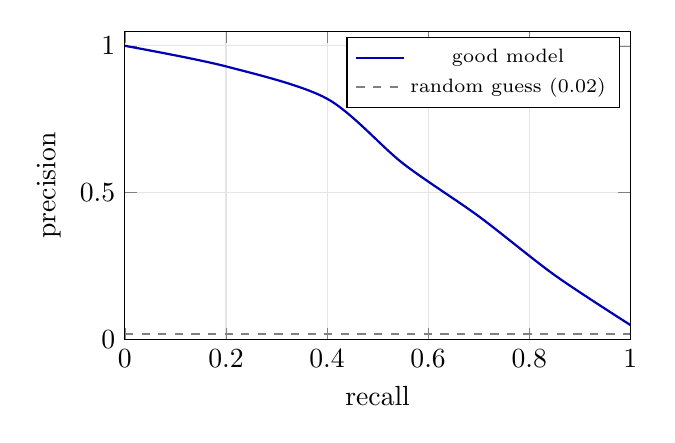
\begin{tikzpicture}
\begin{axis}[width=8cm,height=5.5cm,xlabel={recall},ylabel={precision},xmin=0,xmax=1,ymin=0,ymax=1.05,
  legend style={font=\scriptsize,at={(0.98,0.98)},anchor=north east},grid=major,grid style={black!10}]
\addplot[blue!70!black,thick,smooth] coordinates {(0,1)(0.2,0.93)(0.4,0.82)(0.55,0.6)(0.7,0.42)(0.85,0.22)(1,0.05)};
\addlegendentry{good model}
\addplot[black!50,dashed,thick] coordinates {(0,0.02)(1,0.02)};
\addlegendentry{random guess (0.02)}
\end{axis}
\end{tikzpicture}
\caption{Illustrative PR curve. The area under the blue line is the PR-AUC.}
\end{figure}

\textbf{Why PR and not ROC:} the ROC curve uses the false-alarm rate, whose denominator is the huge number of normal
days, so even many false alarms look small and ROC-AUC looks excellent for weak models. PR-AUC focuses on the rare
class, which is the one that matters.

\section{The three test subsets}
\begin{itemize}
  \item \textbf{All days:} every test row (1,932,437 rows, 37,450 extreme).
  \item \textbf{Severe:} all normal rows plus only the 10\% most severe extreme rows (largest $z$). It asks: can the
        model catch the worst heat? This is the main score of the project.
  \item \textbf{Onset:} only rows where today's maximum is still below tomorrow's threshold. The model cannot simply
        say ``hot today, so hot tomorrow''; it must predict the \emph{start} of an extreme.
\end{itemize}

\section{Per-seed mean vs combined model}
Each setting is trained with 5 seeds. The \textbf{per-seed mean} averages the 5 scores (it shows how consistent the
gain is, and ``runs better'' counts how many of the 5 seeds beat real-only). The \textbf{combined (ensemble)} score
averages the 5 predicted probabilities first and scores that; it is a little higher, and is what you would use in
practice.

\begin{sayit}
``Accuracy is meaningless when 98\% of days are normal, so I use PR-AUC, the area under the precision--recall curve.
Random guessing scores 0.02. I report it on all days, on the most severe 10\% of extremes, and on onset days.''
\end{sayit}
